\begin{marginfigure}
\begin{tikzpicture}
\node [name-dest] (box){%
    \begin{minipage}{0.80\textwidth}
     \begin{itemize}
    \item Rhys Tyers
    \item David Kirkpatrick
    \end{itemize}
    \end{minipage}

};
\node[fancytitle, right=10pt] at (box.north west) {Xanadon't};
\end{tikzpicture}
\end{marginfigure}

\section{The mighty Xanadon't traverse}
 
We'd just woken up. The fairy lights strung across the wall cast a dim white glow across our camp. Packets of Smash, noodles and a bewildering variety of soup lay scattered across the floor, daring us to combine them into  a homogeneous breakfast goop.The little stove, surrounded by half used and identical plastics bags of sugar and dried milk, was already roaring, producing the first of many pans of tea. We sat huddled in sleeping bags and fleece pajamas listening to hit songs of the eighties echo off the rock around us.


\begin{marginfigure}
\frame{\includegraphics[width=\linewidth]{"images/2013/rhys-xanadont-2013/camp-X-Ray_in_full_swing".png}}
\label{}
\caption{Camp \protect\passage{X-Ray} in full swing --- Iztok Mozir}
\end{marginfigure}
It's comfortable in camp, despite being 500 metres below the surface, and leaving is always hard. Dave and I had a plan though. A plan that would surely bring us glory and riches. So we shed our warm fleece and retrieved our damp wetsocks, furries and oversuits from the optimistic washing line that runs across the chamber. The damp, near freezing air that breezes through is not interested in drying our gear but we hang it up all the same, hoping that by some osmotic miracle we wake to dry clothes. Suited up, with a bag full of metal, rope and an overclocked Ikea drill we set off.

\margininbox{The plan}{

`After much faffing and two dinners we are finally getting ready for bed. Dave and I had a 6 hour ``push'' in which we found a bypass to the \protect\passage{Euphrates} super grim crawl that pops out in \protect\passage[Big Rock Candy Mountain]{Big Rock}. Tomorrow we intend to construct the \protect\passage{Xanadon't} traverse to access it. I will be drilling and Dave will presumably be complaining.'
\protect\mininame{Rhys Tyers}

`I dreamt about rocks.'
\protect\mininame{David Kirkpatrick}
}

The day before Dave and I had been in a promising bit of cave named \passage{Cuckoo's Nest}, a tall, dry and winding phreatic passage. We hadn't found the way to the main pushing front and had instead spent some time poking around every moderately human sized hole that the previous team may have missed. Towards the end of our trip, with no significant new passage to our name, I climbed up into a sandy chamber and followed a low crawl. My helmet scraped along the ceiling as I dragged myself past the final constriction to be greeted by nothing. The crawl flanged out into vast, inky blackness. I could barely contain my excitement, the prospect of a big new pitch all to myself was too much. I leaned tentatively out into the darkness and examined my new discovery. 

The bottom was lost in the depths and the far wall was only just visible. I turned to my left, and my heart sank. A rope. The thin white record of previous cavers dangled down, mocking. I recognized it fairly quickly, the only nearby large pitch was \passage{Big Rock Candy Mountain}, this must be a window into it. I scrambled back to Dave to tell him of my finding. Despite the let down this was still good news. The previous route to \passage{Cuckoo's Nest} was an awkward rift traverse followed by the most unpleasant muddy, wet, draughty crawl known to man. If we could rig a bypass down to the window I had found the new route would be an easy walk from camp, saving much time and psychological trauma for future explorers.

\begin{pagefigure}
\frame{\includegraphics[width=\linewidth]{"images/2013/rhys-xanadont-2013/rhys_hard_work".jpg}}
\label{}
\caption{Rhys hard at work --- Kate Smith}
\end{pagefigure}

So here we were, to rig the bypass. At the top of \passage{Big Rock Candy Mountain}, Dave and I set up a forward base. We had brought a gas stove, tea and as much marzipan and ginger cake as we could cram into a tackle sack. As the competent and confident caver of two years caving experience I was going to go down first. 

My plan was to rig a traverse from a rebelay I saw from the window. I grabbed a bag of rope and slung the drill strap around my shoulders and descended. The pitch wall is mostly an interesting combination of mud and flakes, neither of which are ideal for a bolt. After some swinging though I found a clean, solid looking face to bolt. I lined up the drill and pulled the trigger. The high pitched whine and dusty spray flying from the drill were satisfying and soon the drill bit was smoothly disappearing into the rock. The drill slowed, the whine turned to a grind and finally it sputtered a few angry clicks at me and stopped. 

I tried again, and again, and again. But the same each time, whine, grind, click, stop. Each time stopping faster until the drill would no longer spin. The battery must be dead, I thought, and climbed back up to Dave. A minor inconvenience at the most we thought and returned to camp to retrieve the spare battery. A while later I was back, inserting the drill into my half finished hole, a new block of chemical energy clenched between my thighs. But again the drill refused to cooperate. Whine, grind, click, stop. 

The drill must be fucked, I thought and climbed back up to Dave. A second inconvenience but we were not going to be deterred by shoddy Swedish engineering and again trudged back to camp to retrieve the hand bolting kit. 

\begin{pagefigure}
\centering
\begin{subfigure}[t]{0.49\textwidth}
\frame{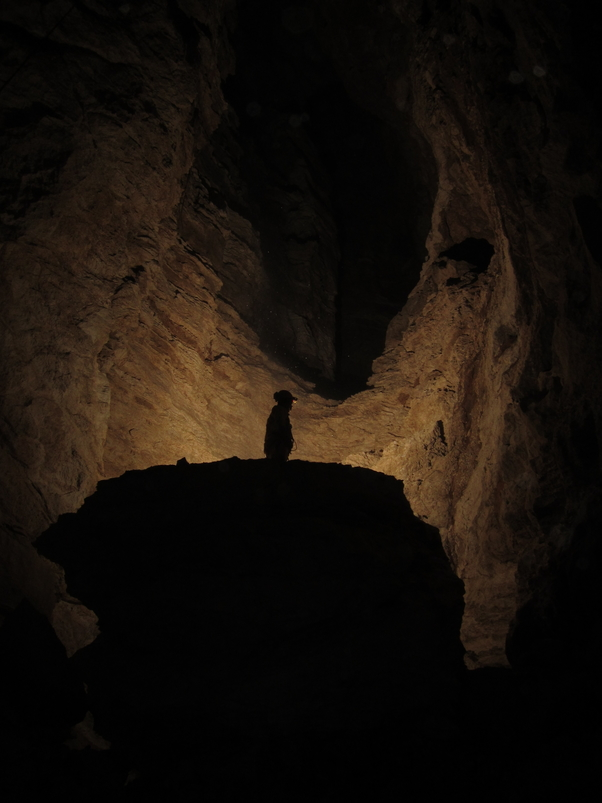
\includegraphics[width=\linewidth]{images/2013/rhys-xanadont-2013/bottom_big_rock_1.jpg}}
\caption{}
\end{subfigure}
\hspace{2pt}
\begin{subfigure}[t]{0.49\textwidth}
\frame{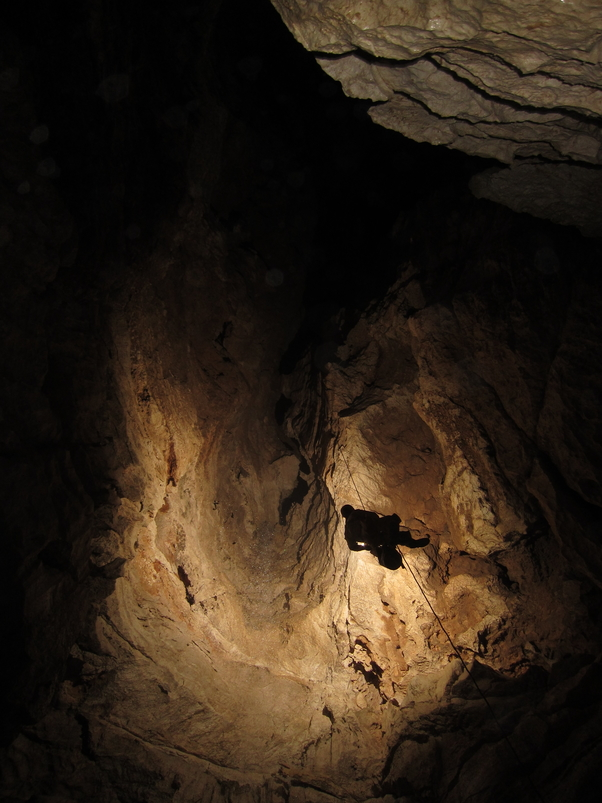
\includegraphics[width=\linewidth]{images/2013/rhys-xanadont-2013/bottom_big_rock_2.jpg}}
\caption{}
\end{subfigure}
\caption{\protect\passage{Big Rock Candy Mountain} ( named after the massive boulder in \textbf{(a)}) is a twin pitch located at the end of \protect\passage{Friendship Gallery}, over which it is now possible to traverse to reach the \protect\passage{Cuckoo's Nest} extensions --- Jarvist Frost}
\label{none}
\end{pagefigure}

Back at the now familiar spot, the half drilled hole staring at me, I wielded hammer and driver and got to work. I might whine, the driver might grind, the hammer might click but we would not stop. 

Tap, tap, tap. Tap, tap, tap. Tap, tap, tap. The clinking of the hammer against the driver calmed me into the familiar bolting rhythm. 

Tap, tap, tap. Tap, tap, tap. Almost done. 

Tap, tap, tap. Tap, tap, tap. Tap, tap, crack. 

Tap, tap, crack? 

I looked at my almost complete bolt. A crack had emerged from it and ran a few millimetres into the rock. Bollocks. I started again. But like my attempts with the drill, the second time was no better. Another crack halfway through bolting. Defeated, I climbed back up. We would need to regroup.

As I reached the top of the pitch something caught my eye. A row of bolts running across the top of the pitch. They would get us more than half the horizontal distance we needed! A miracle I thought as I got off the pitch. In front of me was a glowing silvery spirit, shaking and muttering about thrones and glory. Was this the deity that had placed the bolts? 

No, no, squinting my eyes revealed Dave's face under layers of silver survival blanket, clutching a pathetic tea light for warmth. `I have built a throne' he declared, through chattering teeth. And scuttered further back into the passage. I followed and Dave lead to a large pile of rocks. It's similarity to a throne stopped at `not being the floor' but Dave sat atop it proud as any regent had ever been. I decided it was probably Dave's turn to do some rigging and sent him to rig the mysterious bolts. I sat, drank some tea, ate some ginger cake and prepared for a long wait. I hoped I would be spared the madness that had overcome Dave.



Some time later I heard footsteps approaching. Was someone here to take my throne? My kingdom with its silver sky and single flame! The sky moved and Dave's face loomed over me.  `I rigged it' he says as my cognisance returned. I shivered my way out of the remaining foil and handed the tea light to Dave. Without the heat of the tea light or recent movement I made my way to Dave's new traverse, eager to get to the end and bolt the cold away. I vibrated along it, still none the wiser as to its creator. 

We would later find out that someone else also tried to reach a window in \passage[|see{Big Rock Candy Mountain}]{Big Rock} (a different one) but had failed, leaving these bolts behind. Their effort would not be in vain. From the end of the traverse I reckoned I was just two or three bolts away from reaching the window and emboldened by this thought I began once more. The rock here proved strong enough to hold my bolts and I at last I could see the window. I swung over and clipping my cowstail to a flake to hold myself in place, I started the final bolt. This final hang needed to be right over the window so that I could swing in, but to reach the ideal bolt position I had to lean out sideways and stretch out with the hammer. \bignote{Soon my arms were quivering with the exertion and I had to rest}. I was tired and the bolt was barely started. I hung for a while. So close yet so far. As my faith wavered and I considered turning back.

But then Dave called out. He was behind me. He had descended the original pitch and was now visible, on the other side. Stirred by companionship I bolted once more. It was slow going. Several times I shouted that I wanted to give up but Dave's friendly words reverberated around me. Sometimes he offered encouragement, mostly he complained about the position of his genitals within his harness. 

With a final tap I decided the bolt was secure and lowered myself into the window. Dave came across to examine the new route, finding me collapsed in the sand. Our quest complete, and eager to claim the praise and applause we would surely received, we returned to camp.

\name{Rhys Tyers}
